\documentclass[14pt]{extarticle}
\usepackage{fontspec}
\usepackage{polyglossia}
\usepackage{amsmath}
\usepackage{amssymb}
\usepackage{xcolor}
\usepackage{fancyhdr}
\usepackage{graphicx}
\usepackage{listings}
\usepackage[most]{tcolorbox}
% \usepackage{setspace}
\usepackage{pifont}
\usepackage{enumitem}
\usepackage{titlesec}
\usepackage[bottom]{footmisc}
\usepackage{titling}
\usepackage{minted}
\usepackage{etoolbox}
\usepackage{array}
\usepackage{extsizes}
\usepackage{float}
\usepackage{booktabs}
\usepackage{hyperref}
\usepackage[onehalfspacing]{setspace}
\usepackage[a4paper, top=2.7cm, bottom=2.7cm, left=2.5cm, right=2.5cm, headheight=1.5cm, headsep=0.5cm]{geometry}
\usepackage{tikz}

\usetikzlibrary{automata, positioning, arrows.meta, arrows}

\newfontfamily\emoji{Segoe UI Emoji}

\pagestyle{fancy}

\setmainlanguage[numerals=western]{arabic}
\setotherlanguage{english}
% \newfontfamily\arabicfont[Script=Arabic]{Amiri}
\newfontfamily\arabicfont[Script=Arabic]{Calibri}
\newfontfamily\arabicfonttt[Script=Arabic]{Courier New}

\lstset{
  language=[Sharp]C,
  numbers=left,
  stepnumber=1,
  numbersep=8pt,
  frame=single,
  basicstyle=\ttfamily\small,
  keywordstyle=\color{blue},
  stringstyle=\color{red},
  commentstyle=\color{green!50!black}
}

\newif\ifdetailed
\ifdefined\setdetailed
  \setdetailed
\fi

\newif\ifwithsols
\ifdefined\setwithsols
  \setwithsols
\fi

% unified tcolorboxes for articles
\tcbset{colback=white, colframe=black, fonttitle=\bfseries, boxrule=0.8pt}
\newtcolorbox{boxDef}[1][]{colback=blue!5!white,colframe=blue!75!black,
  title={{\emoji📘} تعريف\ifx\\#1\\\else ~#1\fi :}}
\newtcolorbox{boxExercise}[1][]{colback=cyan!5!white,colframe=cyan!70!black,
  title={{\emoji🧩} تمرين\ifx\\#1\\\else ~#1\fi :}}
\newtcolorbox{boxExample}[1][]{colback=yellow!5!white,colframe=orange!90!black,
  title={{\emoji📝} مثال\ifx\\#1\\\else ~#1\fi :}}
\newtcolorbox{boxNote}[1][]{colback=gray!10!white,colframe=black,
  title={{\emoji✨} ملاحظة\ifx\\#1\\\else ~#1\fi :}}
\newtcolorbox{boxAttention}[1][]{colback=magenta!10!white,colframe=magenta!80!black,
  title={{\emoji🔔} تنبيه\ifx\\#1\\\else ~#1\fi :}}
\newtcolorbox{boxWarning}[1][]{colback=red!5!white,colframe=red!75!black,
  title={{\emoji⚡} ملاحظة هامة\ifx\\#1\\\else ~#1\fi :}}
\newtcolorbox{boxSolution}[1][]{colback=green!5!white,colframe=green!60!black,
  title={{\emoji✅} حل\ifx\\#1\\\else ~#1\fi :}}
\newtcolorbox{boxSymbol}[1][]{colback=purple!5!white,colframe=purple!70!black,
  title={{\emoji🔣} رمز\ifx\\#1\\\else ~#1\fi :}}
\newtcolorbox{boxHint}[1][]{colback=teal!5!white,colframe=teal!60!black,
  title={{\emoji💡} تلميح\ifx\\#1\\\else ~#1\fi :}}


\tcbset{simplecode/.style={ colback=gray!5, colframe=black!50, boxrule=0.4pt, arc=2pt, left=4pt,right=4pt,top=4pt,bottom=4pt}}
\newenvironment{boxCode}{\begin{tcolorbox}[simplecode]}{\end{tcolorbox}}

\newcolumntype{C}[1]{>{\centering\arraybackslash}p{#1}}

% redefine spaces after titles
\makeatletter
\renewcommand{\@maketitle}{%
  \begin{center}
    {\huge \bfseries \@title \par}%
    \vskip 0.2em % space between title and author
    {\large \@author \par}%
    % \vskip 0.2em % space between author and date
    % {\normalsize \@date \par}%
  \end{center}
}
\makeatother

\fancyhf{} % clear default
\fancypagestyle{plain}{
  \fancyhf{}
  \fancyhead[L]{مدرسة التسامح الشاملة}
  % \fancyhead[L]{
\includegraphics[height=1cm]{../../../images/logoTasamoh.png}}
  \fancyhead[R]{الأستاذ محمود اغبارية}
  \fancyfoot[C]{\thepage}
}

\fancyhead[L]{مدرسة التسامح الشاملة}
\fancyhead[R]{الأستاذ محمود اغبارية}
\fancyfoot[C]{\thepage}
% \date{\today}

\setcounter{tocdepth}{3} % only section subsection and subsubsection in TOC

\newcommand{\importpdfpage}[2]{%
    \thispagestyle{empty}
    \newgeometry{left=0cm,right=0cm,top=0cm,bottom=0cm}
    \includegraphics[page=#2,width=0.95\paperwidth,height=0.95\paperheight,keepaspectratio]{#1}
    \restoregeometry
}

\newcommand{\insertFullImg}[1]{%
    \noindent
    \makebox[\textwidth][c]{
        \includegraphics[width=0.9\paperwidth,keepaspectratio]{#1}%
    }%
}%

% ----------------------


% \begin{document}

% \maketitle

% % \clearpage  % start TOC on a new page
% % \renewcommand{\contentsname}{جدول المحتويات}
% % \tableofcontents
% % \clearpage

% \part*{part 1} % the * prevents numbering
% \section*{مقدمة}
% \subsection*{مثال رياضي}
% \subsubsection*{مثال فرعي}
% \paragraph*{ paragraph 1}
% \subparagraph*{sub paragraph 1}

% \ifdetailed
% \begin{english}
% \begin{minted}{csharp}
% // C# Example
% \end{minted}
% \end{english}
% \fi

% OLD WAY
% \ifdetailed
% \begin{english}
% \begin{lstlisting}
% // C# Example
% \end{lstlisting}
% \end{english}
% \fi

% % 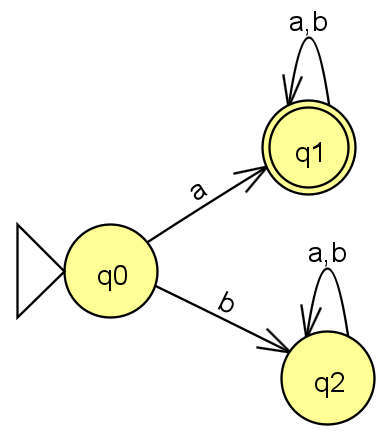
\includegraphics[width=0.2\textwidth]{../../../images/DFAs/ex1_q1.png}



% \vspace{3cm}
% \begin{flushleft}
% أرجو لكم وقتًا ممتعًا.

% الأستاذ محمود اغبارية.
% \end{flushleft}


% \end{document}


\ifwithsols
\title{حل وظيفة 17 - ترتيب الإدخال}
\else
\title{وظيفة 17 - ترتيب الإدخال}
\fi

\begin{document}

\maketitle
\thispagestyle{fancy}

\textbf{للتذكير، هذا هو كود ترتيب الإدخال:}
\begin{english}
\begin{boxCode}
\begin{minted}{csharp}
public static void InsertionSort(int[] arr)
{
    for (int i = 1; i < arr.Length; i++)
    {
        int key = arr[i];
        int j = i - 1;
        while (j >= 0 && arr[j] > key)
        {
            arr[j + 1] = arr[j];
            j--;
        }
        arr[j + 1] = key;
    }
}
\end{minted}
\end{boxCode}
\end{english}

\clearpage

\begin{enumerate}[itemsep=3em]
    \item نعرّف المصفوفات التالية:
\begin{english}
\begin{boxCode}
\begin{minted}{csharp}
int[] arr1 = {9, 3, 7, 1, 5};
int[] arr2 = {1, 2, 3, 4, 5};
int[] arr3 = {10, 9, 8, 7, 6};
\end{minted}
\end{boxCode}
\end{english}
لكل واحدة من المصفوفات أعلاه طبّق خوارزمية \textenglish{InsertionSort}
 خطوة بخطوة، واملأ الجدول التالي الذي يُبيّن حالة كل مصفوفة بعد انتهاء كل دورة \textenglish{i}:

\begin{center}
\begin{tabular}{|c|c|c|c|}
\hline
 & \multicolumn{3}{c|}{\textbf{قيمة المصفوفة في نهاية الدورة \textenglish{i}}} \\
\cline{2-4}
\textbf{قيمة \textenglish{i}} & \textbf{المصفوفة \textenglish{arr1}} & \textbf{المصفوفة \textenglish{arr2}} & \textbf{المصفوفة \textenglish{arr3}} \\
\hline
\textenglish{i = 1} & \hspace{3.5cm} & \hspace{3.5cm} & \hspace{3.5cm} \\[15pt]
\hline
\textenglish{i = 2} & & & \\[15pt]
\hline
\textenglish{i = 3} & & & \\[15pt]
\hline
\textenglish{i = 4} & & & \\[15pt]
\hline
\end{tabular}
\end{center}

\ifwithsols
\begin{boxSolution}
\begin{center}
\renewcommand{\arraystretch}{1.5}
\begin{tabular}{|c|c|c|c|}
\hline
 & \multicolumn{3}{c|}{\textbf{قيمة المصفوفة في نهاية الدورة \textenglish{i}}} \\
\cline{2-4}
\textbf{قيمة \textenglish{i}} & \textbf{المصفوفة \textenglish{arr1}} & \textbf{المصفوفة \textenglish{arr2}} & \textbf{المصفوفة \textenglish{arr3}} \\
\hline
\textenglish{i = 1} & \textenglish{\{3, 9, 7, 1, 5\}} & \textenglish{\{1, 2, 3, 4, 5\}} & \textenglish{\{9, 10, 8, 7, 6\}} \\
\hline
\textenglish{i = 2} & \textenglish{\{3, 7, 9, 1, 5\}} & \textenglish{\{1, 2, 3, 4, 5\}} & \textenglish{\{8, 9, 10, 7, 6\}} \\
\hline
\textenglish{i = 3} & \textenglish{\{1, 3, 7, 9, 5\}} & \textenglish{\{1, 2, 3, 4, 5\}} & \textenglish{\{7, 8, 9, 10, 6\}} \\
\hline
\textenglish{i = 4} & \textenglish{\{1, 3, 5, 7, 9\}} & \textenglish{\{1, 2, 3, 4, 5\}} & \textenglish{\{6, 7, 8, 9, 10\}} \\
\hline
\end{tabular}
\end{center}
\end{boxSolution}
\clearpage
\fi

\item
اكتب عملية خارجية \textenglish{InsertionSortDescending} تتلقى مصفوفة أعداد صحيحة \textenglish{arr} وترتّبها \textbf{تنازلياً} (من الأكبر إلى الأصغر).

\ifwithsols
\begin{boxSolution}
\begin{english}
\begin{boxCode}
\begin{minted}{csharp}
public static void InsertionSortDescending(int[] arr)
{
    for (int i = 1; i < arr.Length; i++)
    {
        int key = arr[i];
        int j = i - 1;
        // we change the condition here to arr[j] < key
        while (j >= 0 && arr[j] < key)
        {
            arr[j + 1] = arr[j];
            j--;
        }
        arr[j + 1] = key;
    }
}
\end{minted}
\end{boxCode}
\end{english}
\textbf{الشرح:} التغيير الوحيد عن الترتيب التصاعدي هو في شرط الـ \textenglish{while}: \\
 نغيّر \textenglish{arr[j] > key} إلى \textenglish{arr[j] < key}، لأننا نريد إزاحة العناصر \textbf{الأصغر} لليمين.
\end{boxSolution}
\clearpage
\fi

\end{enumerate}

\vspace{1cm}
\begin{flushleft}
أرجو لكم عملاً ممتعاً!

الأستاذ محمود اغبارية.
\end{flushleft}

\end{document}